\documentclass[12pt,letterpaper]{article}
\usepackage{graphicx,textcomp}
\usepackage{natbib}
\usepackage{setspace}
\usepackage{fullpage}
\usepackage{color}
\usepackage[reqno]{amsmath}
\usepackage{amsthm}
\usepackage{fancyvrb}
\usepackage{amssymb,enumerate}
\usepackage[all]{xy}
\usepackage{endnotes}
\usepackage{lscape}
\newtheorem{com}{Comment}
\usepackage{float}
\usepackage{hyperref}
\newtheorem{lem} {Lemma}
\newtheorem{prop}{Proposition}
\newtheorem{thm}{Theorem}
\newtheorem{defn}{Definition}
\newtheorem{cor}{Corollary}
\newtheorem{obs}{Observation}
\usepackage[compact]{titlesec}
\usepackage{dcolumn}
\usepackage{tikz}
\usetikzlibrary{arrows}
\usepackage{multirow}
\usepackage{xcolor}
\newcolumntype{.}{D{.}{.}{-1}}
\newcolumntype{d}[1]{D{.}{.}{#1}}
\definecolor{light-gray}{gray}{0.65}
\usepackage{url}
\usepackage{listings}
\usepackage{color}

\definecolor{codegreen}{rgb}{0,0.6,0}
\definecolor{codegray}{rgb}{0.5,0.5,0.5}
\definecolor{codepurple}{rgb}{0.58,0,0.82}
\definecolor{backcolour}{rgb}{0.95,0.95,0.92}

\lstdefinestyle{mystyle}{
	backgroundcolor=\color{backcolour},   
	commentstyle=\color{codegreen},
	keywordstyle=\color{magenta},
	numberstyle=\tiny\color{codegray},
	stringstyle=\color{codepurple},
	basicstyle=\footnotesize,
	breakatwhitespace=false,         
	breaklines=true,                 
	captionpos=b,                    
	keepspaces=true,                 
	numbers=left,                    
	numbersep=5pt,                  
	showspaces=false,                
	showstringspaces=false,
	showtabs=false,                  
	tabsize=2
}
\lstset{style=mystyle}
\newcommand{\Sref}[1]{Section~\ref{#1}}
\newtheorem{hyp}{Hypothesis}

\title{\textbf{MS Contribution to:} Lee, C. (2019). China’s Energy Diplomacy: Does Chinese Foreign Policy Favor Oil-Producing Countries? Foreign Policy Analysis, 15(4), 570–588. https://doi.org/10.1093/fpa/orz011

}
\date{Due: March 31, 2024}
\author{Applied Stats II \\ \vspace{\baselineskip}
	\textbf{Maiia Skrypnyk 23371609}}

\begin{document}
	\maketitle

\section{Twist 1: Plots}


\textbf{Loading the data:}
\lstinputlisting[language=R, firstline=14, lastline=17]{Twist_Lee_MS.R} 


\noindent \textbf{Figure 2 Twist:}

On p. 581, Lee presents four plots (Figure 2: 'I select four African oil-producing countries that have received Chinese aid (\textbf{Angola, Cameroon, Nigeria, Tunisia }— MS) , and graphically present the amount of aid received and their oil production from 2000 to 2013 in figure 2. As shown in figure 2, Chinese aid (denoted by the solid line) fluctuates from year to year, whereas oil production (denoted by the dashed line) is relatively stable over time. Angola, for example, received more than 2 billion dollars from China in 2005, 2007, and 2011 each but none in 2000 or 2009. In other words, if the time-serial variation is taken into account, the results may be confounded by the volatility of Chinese aid. Because the annual aid amount is subject to the Chinese government’s yearly budget, it is less likely that it will clearly follow aid recipients’ oil production every year. \textit{When I only focus on the variation across African countries, however, it is observed that \textbf{African oil producers in general receive more Chinese aid than non–oil producers.}}.

My idea was to test this last finding, therefore I randomly chose one non-oil producing state from each of the five UN African regions: \textbf{Morocco} from Northern Africa, \textbf{Senegal} from Western Africa, \textbf{Central African Republic} from Central Africa, \textbf{Burundi} from Eastern Africa, and \textbf{Botswana} from Southern Africa, and created similar plots of the amount of Chinese aid receives over their oil production 2000-2013 (which is denoted as 0 in this dataset). I also plotted one other major African oil-producer, Sudan, which was not included in Lee's initial analysis, to compare with the non-oil producers. \textbf{Overall. Lee's findings were proved to be correct: if focused on the variation across African countries, it is indeed observed that African non-oil producers receive notably less Chinese aid that oil-producers. }

\lstinputlisting[language=R, firstline=20, lastline=92]{Twist_Lee_MS.R}  


\begin{figure}[H]
    \centering
    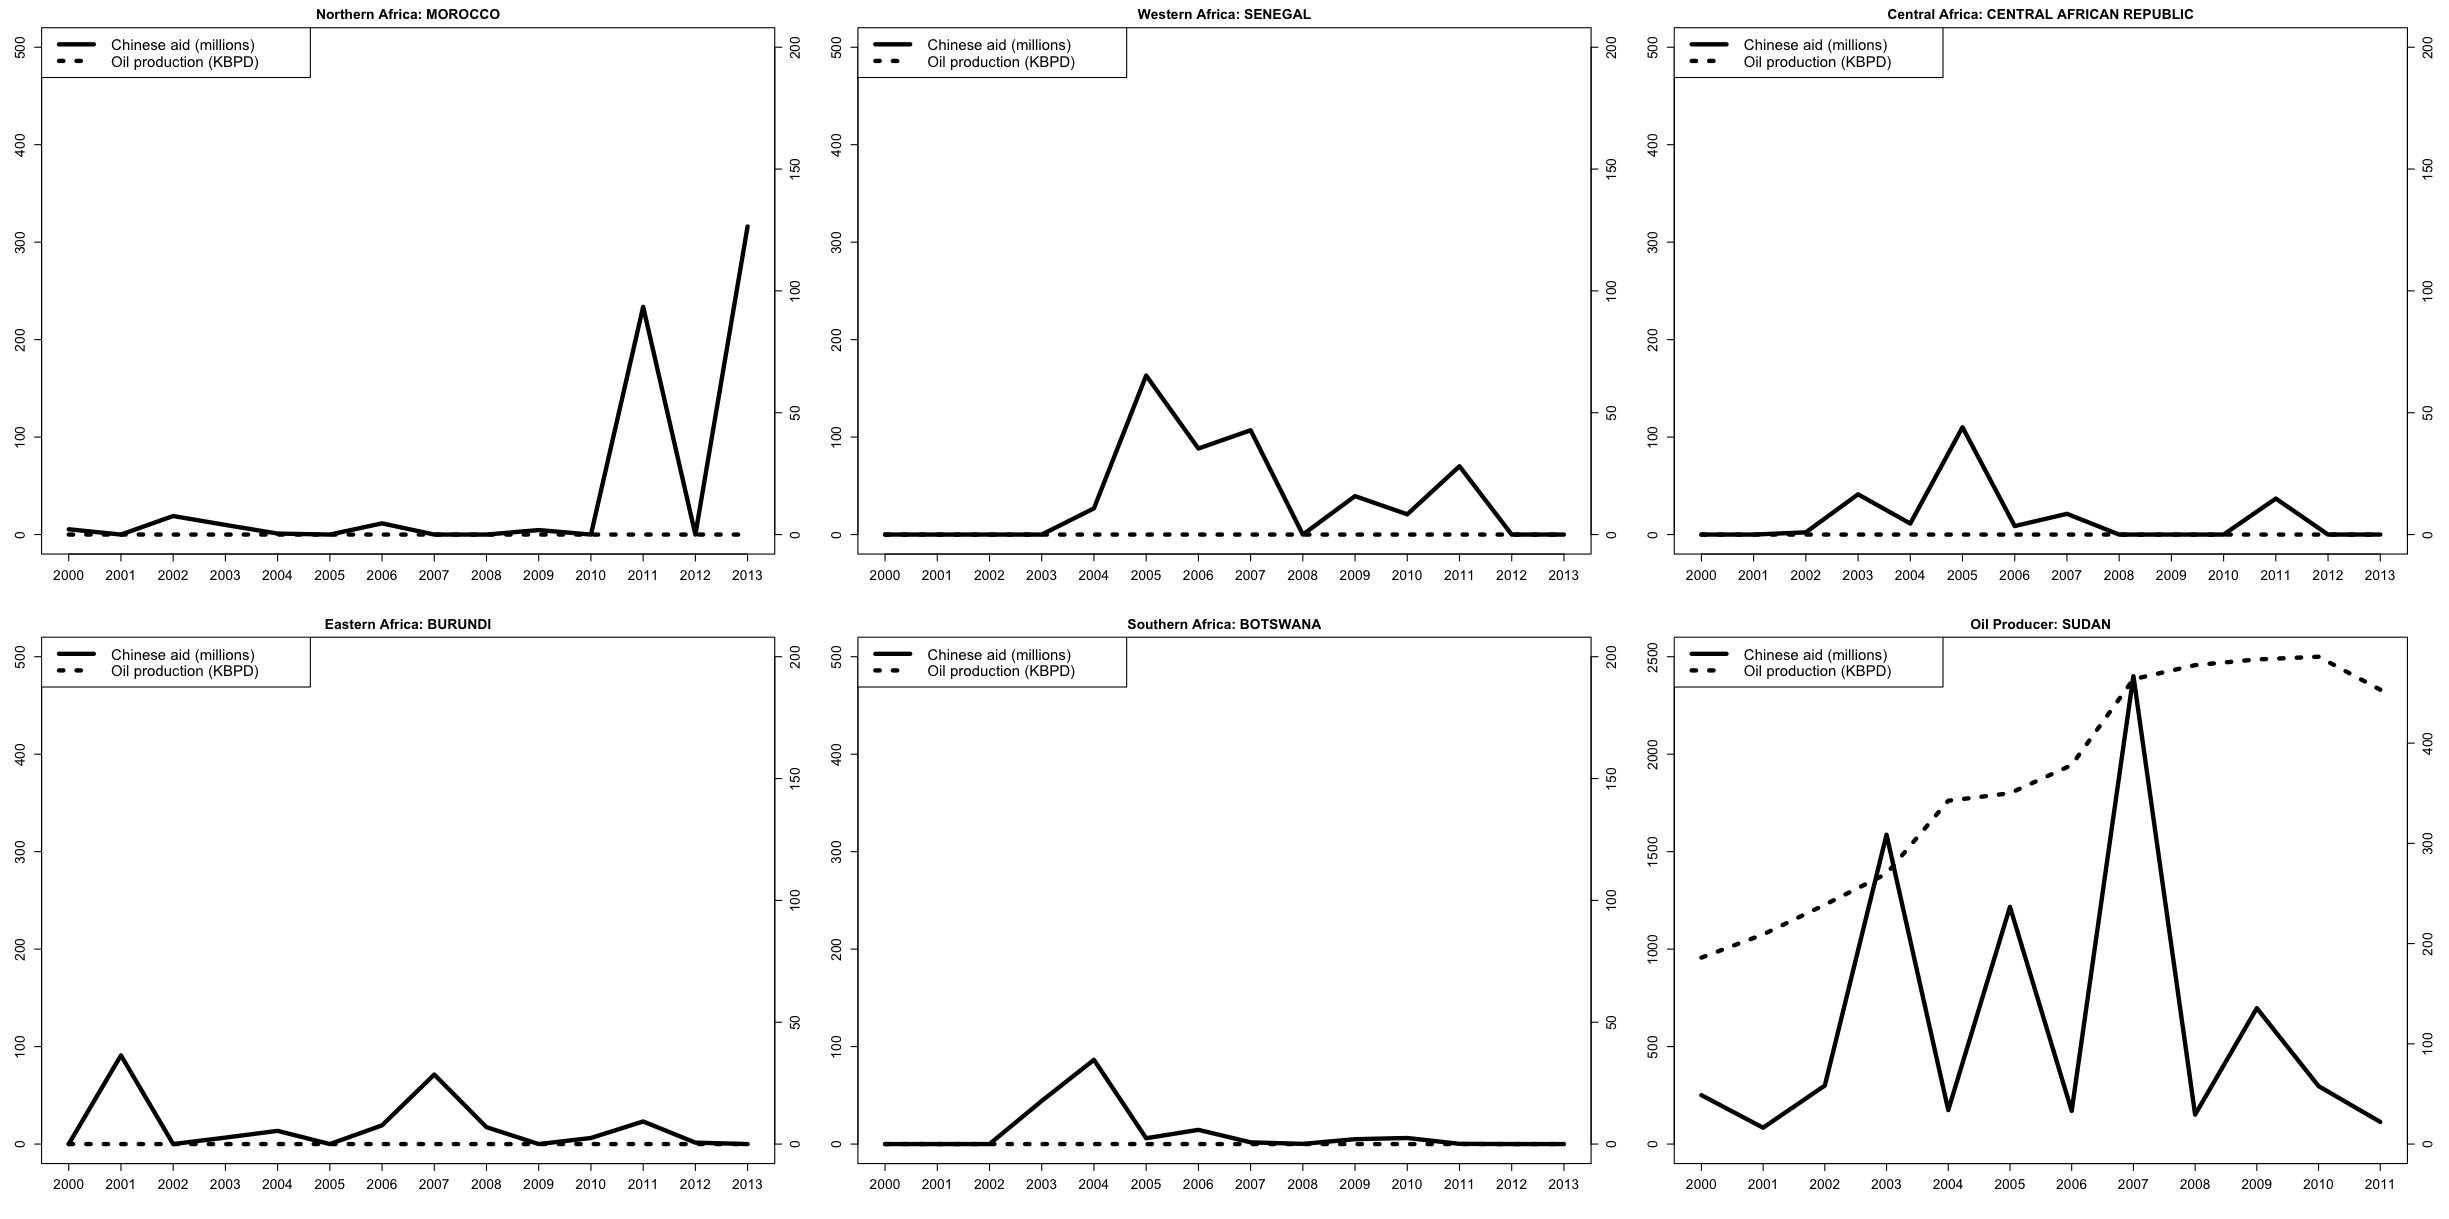
\includegraphics[width=1\linewidth]{figure2MS.png}
\end{figure}

\newpage
\textbf{Model 1 Twist:}

Lee, p. 576: 'To test the first hypothesis (China is more likely to build partnerships with countries abundant in energy resources — MS), I use data on China’s partnerships. Beijing considers three types of partnerships—partnerships, strategic partnerships, and comprehensive strategic partnerships. [...]. A country is coded as 1 as long as it has a partnership connection with China, regardless of the type'
Lee, p. 579-580: '... the sample includes 125 developing countries. Developed countries (i.e., OECD members) are excluded from the sample because their relationships and interactions with China may follow a different pattern. All the independent and control variables enter the model at their mean values between 1992 and 2012.'. 'As can be seen, the coefficient for oil production is positive and statistically significant at the 5 percent level. This means that \textbf{China is more likely to build partnerships with oil-producing countries. }'. 'In other words, energy abundance plays an important role in determining Beijing’s partnership building. In addition to oil production, FDI has a strong, positive effect in models 1 and 2, meaning that \textbf{China is more likely to form partnerships with countries that receive more FDI.} Trade importance is also positively associated with the formation of strategic or comprehensive strategic partnerships (Model 2 — MS). These findings show that \textbf{China’s partnership diplomacy is largely driven by economic considerations.}'.

While original binomial logit Model 1 includes a binary dependent variable on partnership (0, 1), the dataset itself has more detailed data on the type of partnerships that China has with the non-OECD countries. It includes dummy variables for each of the three types of partnerships: \textbf{partnership, strategic partnership, comprehensive strategic partnership.} My understanding is that these types of partnership are following a certain order, though it might not be the case. My idea was to fit an unordered and ordered logit models with the same dependent variable (though relevelled accordingly for each of the models) and predictors, to test whether they would deliver any additional insights or be of better fit to the data. 

I exponentiated the coefficients for all the models for better clarity, and calculated predicted probabilities to fit confusion matrices, which also helped with establishing the accuracy score of the models. I also estimated the models' statistics, such as \textbf{residual deviance} (how much probabilities estimated from our model differ from the observed proportions of successes), \textbf{Akaike Information Criterion} and \textbf{Bayesian Information Criterion} (goodness of fit measures), and performed \textbf{a Brant test} on the ordered model to establish whether the "proportional odds assumption" holds in its case. 

The following conclusions can be driven from my "twist":

\begin{itemize}
    \item New models confirmed the initial findings that China is more likely to build partnerships with countries abundant in
energy resources + it is also driven by economic considerations (significant coefficients for Oil production, FDI inflows, Trade importance).
\item Both new models performed reasonably efficiently as compared to the initial binomial model, though the ordered
model achieved a higher accuracy score and coefficients more similar in value.
\item Parallel Regression Assumption (PRA) holds for the ordered model, which makes it a more adequate fit for the data.
\item Interesting experiment overall, BUT: the original binomial logit Model 1 is still the most accurate → we might assume
that being China’s partner versus not being China’s partner at all carries greater significance compared to being involved
in a specific type of partnership.
\end{itemize}


\lstinputlisting[language=R, firstline=97, lastline=131]{Twist_Lee_MS.R}  

\begin{figure}[H]
    \centering
    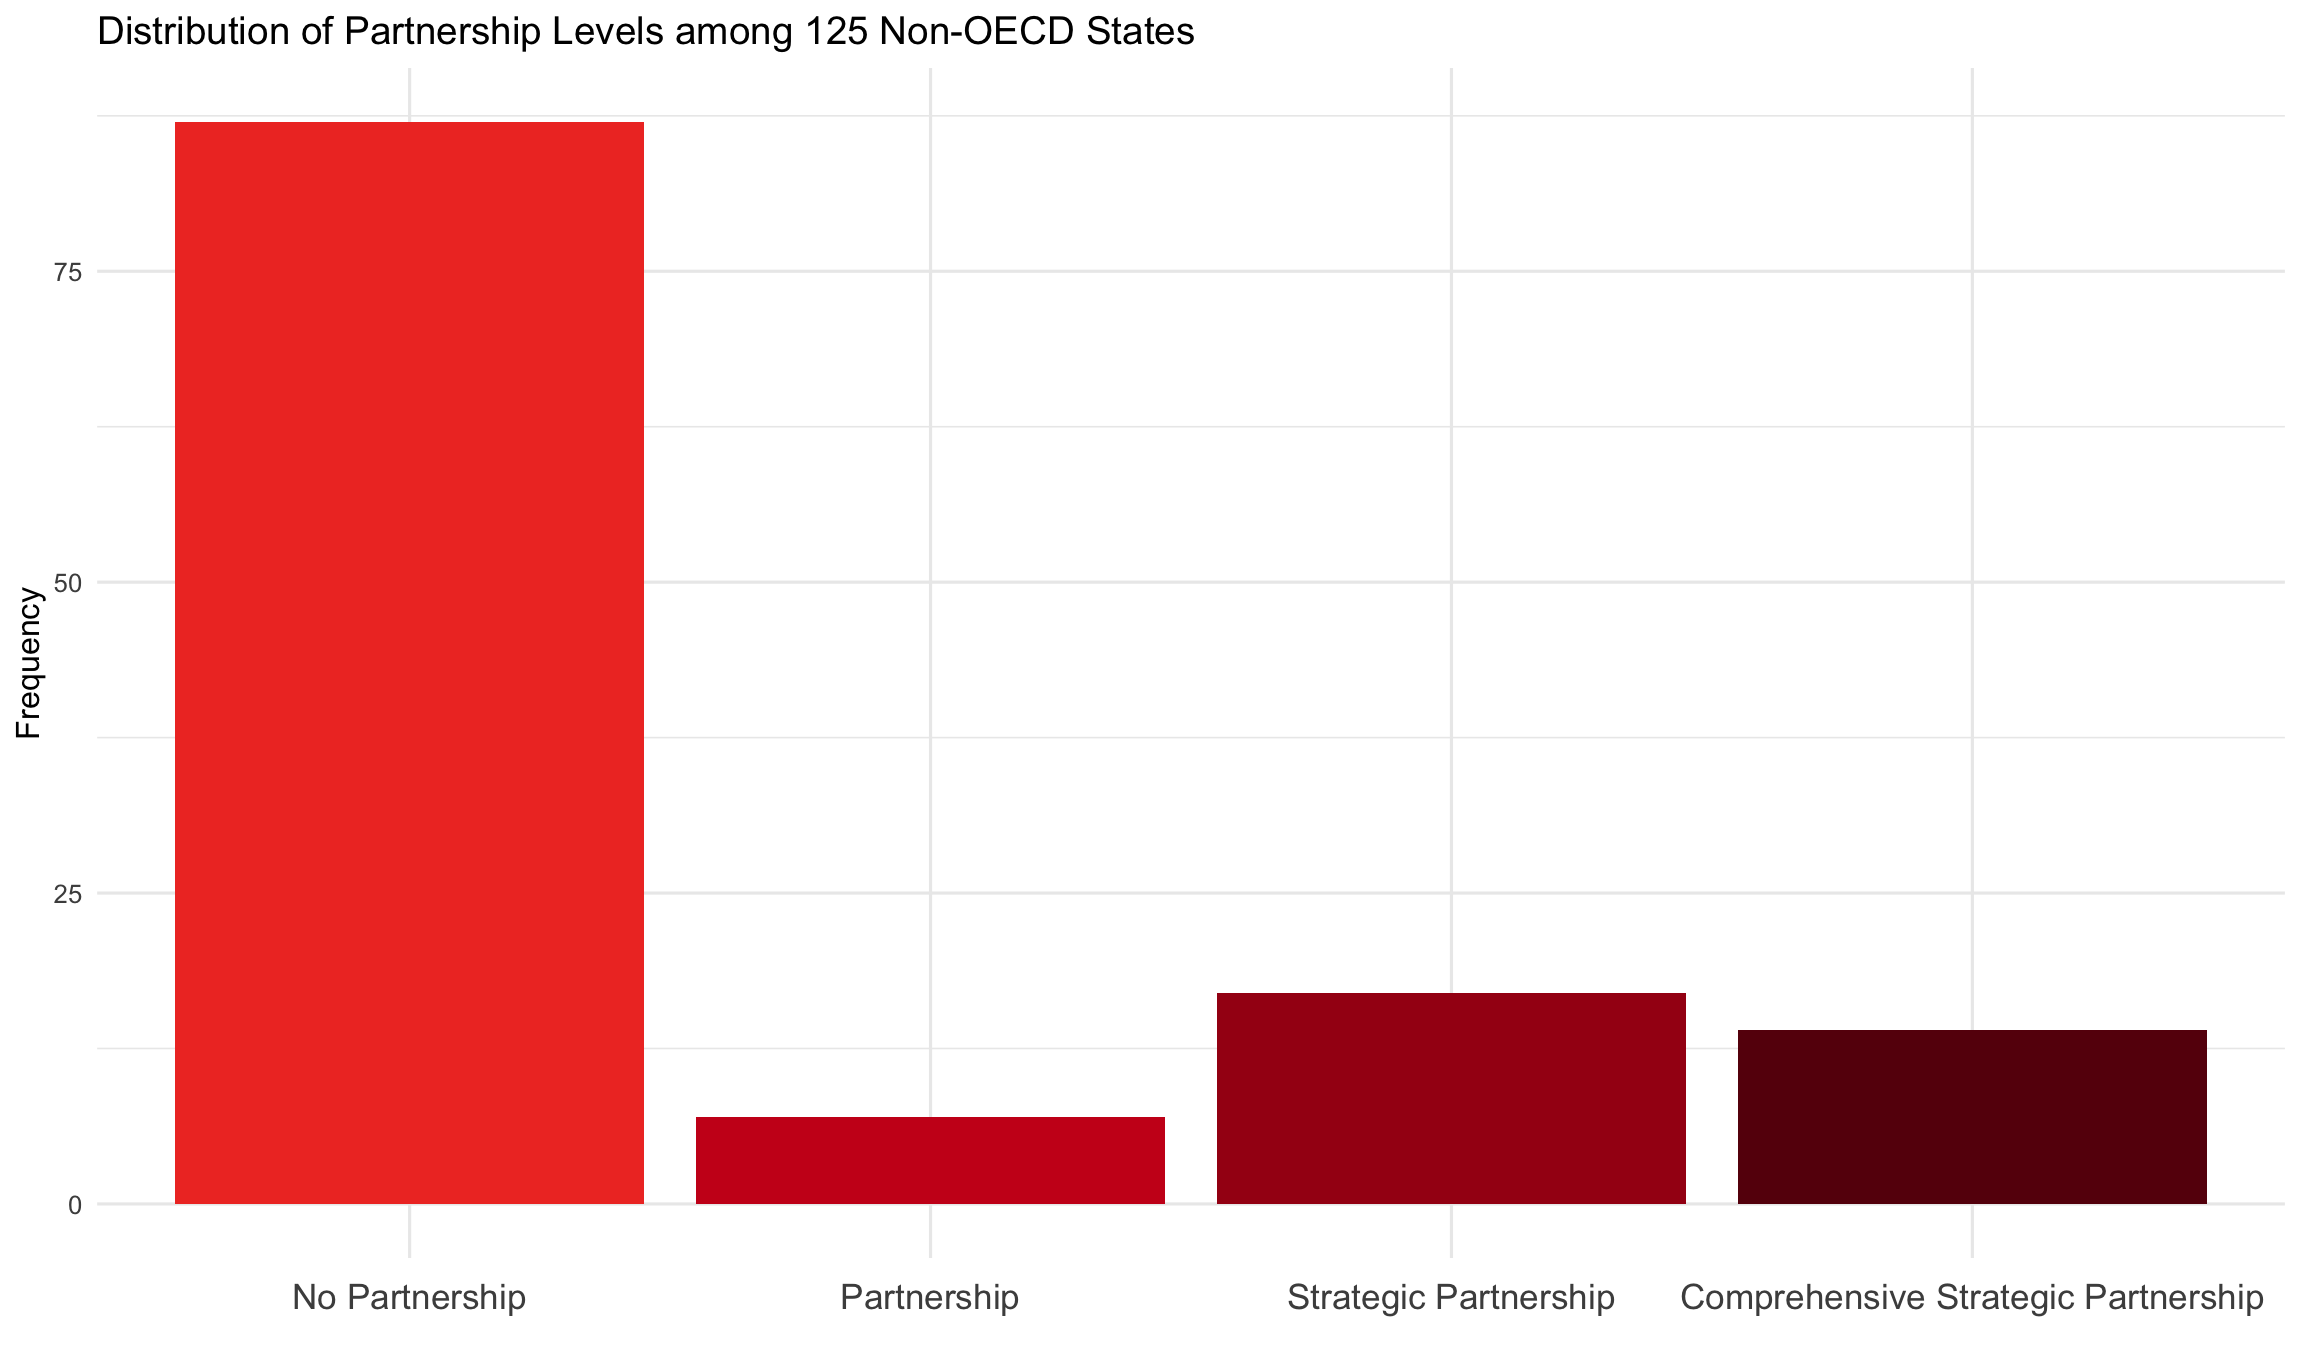
\includegraphics[width=1\linewidth]{plot125.png}
\end{figure}

\lstinputlisting[language=R, firstline=133, lastline=144]{Twist_Lee_MS.R}  

\begin{table}[H] \centering 
  \caption{Original Model 1 (exponentiated)} 
  \label{} 
\begin{tabular}{@{\extracolsep{5pt}}lc} 
\\[-1.8ex]\hline 
\hline \\[-1.8ex] 
 & \multicolumn{1}{c}{\textit{Dependent variable:}} \\ 
\cline{2-2} 
\\[-1.8ex] & Partnership \\ 
\hline \\[-1.8ex] 
 Oil production & 1.139$^{**}$ \\ 
  & (0.058) \\ 
  & \\ 
 GDP per capita & 0.715 \\ 
  & (0.270) \\ 
  & \\ 
 GDP growth & 0.968 \\ 
  & (0.089) \\ 
  & \\ 
 FDI inflows & 1.299$^{***}$ \\ 
  & (0.081) \\ 
  & \\ 
 Trade importance & 3.678 \\ 
  & (0.826) \\ 
  & \\ 
 Level of democracy & 0.993 \\ 
  & (0.051) \\ 
  & \\ 
 Domestic conflict & 1.223 \\ 
  & (0.138) \\ 
  & \\ 
 US ally & 0.398 \\ 
  & (0.777) \\ 
  & \\ 
 Constant & 0.012$^{**}$ \\ 
  & (2.226) \\ 
  & \\ 
\hline \\[-1.8ex] 
Observations & 125 \\ 
Log Likelihood & $-$55.546 \\ 
Residual Deviance & 111.09 \\
AIC & 129.091 \\ 
BIC & 154.5459 \\ 
\hline 
\hline \\[-1.8ex] 
\textit{Note:}  & \multicolumn{1}{r}{$^{*}$p$<$0.1; $^{**}$p$<$0.05; $^{***}$p$<$0.01} \\ 
\end{tabular} 
\end{table} 

\newpage
\lstinputlisting[language=R, firstline=146, lastline=153]{Twist_Lee_MS.R} 

\begin{figure}[H]
    \centering
    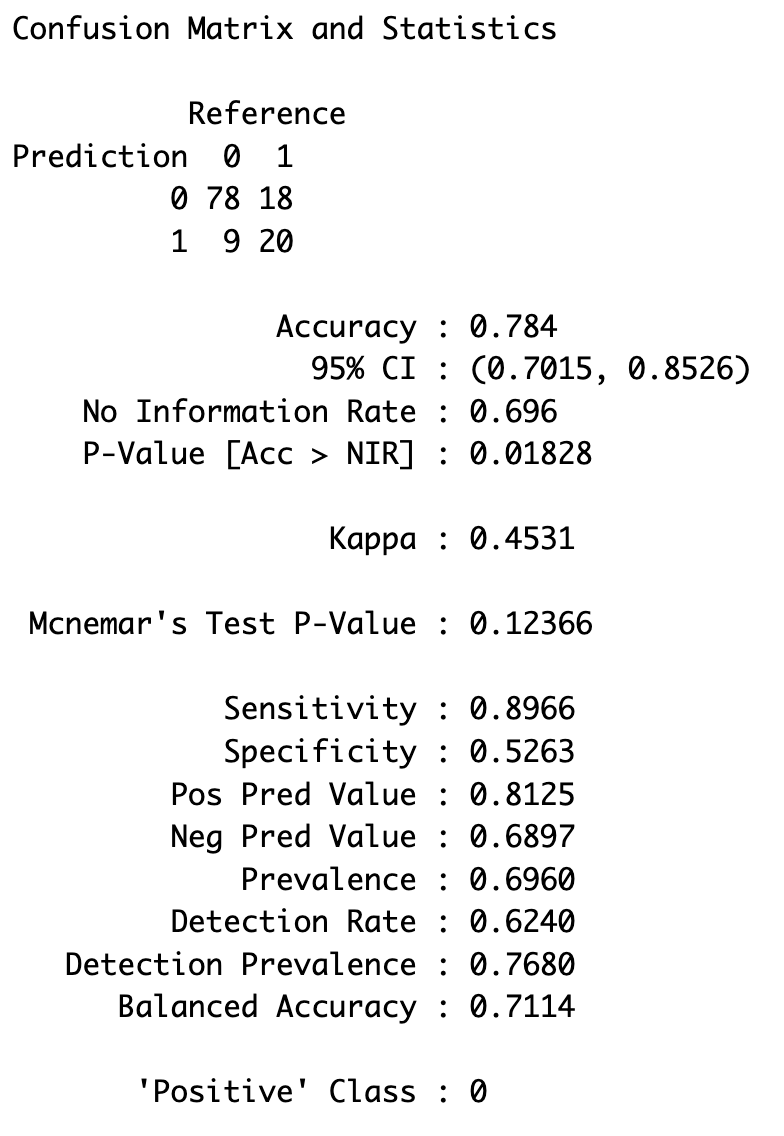
\includegraphics[width=0.5\linewidth]{cm_model1.png}
\end{figure}

\lstinputlisting[language=R, firstline=155, lastline=167]{Twist_Lee_MS.R} 

\begin{figure}[H]
    \centering
    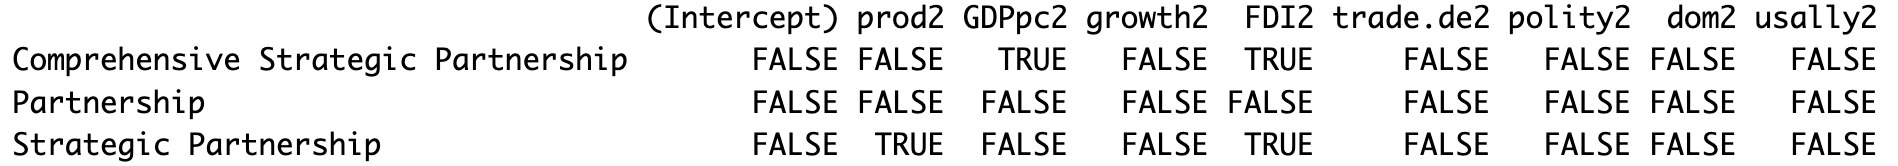
\includegraphics[width=1\linewidth]{pvalues_unord.png}
\end{figure}

\lstinputlisting[language=R, firstline=169, lastline=174]{Twist_Lee_MS.R} 

\begin{table}[H] 
\centering 
\caption{Unordered Model (exponentiated)} 
\label{} 
\begin{tabular}{@{\extracolsep{5pt}}lccc} 
\\[-1.8ex]\hline 
\hline \\[-1.8ex] 
 & \multicolumn{3}{c}{\textit{Dependent variable:}} \\ 
\cline{2-4} 
\\[-1.8ex] & Comprehensive Strategic Partnership & Partnership & Strategic Partnership \\ 
\\[-1.8ex] & (1) & (2) & (3)\\ 
\hline \\[-1.8ex] 
 Oil production & 1.221** & 1.013 & 1.197** \\ 
  & (0.104) & (0.105) & (0.083) \\ 
  & & & \\ 
 GDP per capita & 0.347** & 1.004 & 0.756 \\ 
  & (0.520) & (0.490) & (0.363) \\ 
  & & & \\ 
 GDP growth & 1.003 & 0.864 & 0.980 \\ 
  & (0.157) & (0.227) & (0.103) \\ 
  & & & \\ 
 FDI inflows & 1.885** & 1.133 & 1.266** \\ 
  & (0.284) & (0.148) & (0.097) \\ 
  & & & \\ 
 Trade importance & 10.218** & 0.153 & 2.253 \\ 
  & (1.189) & (4.021) & (1.083) \\ 
  & & & \\ 
 Level of democracy & 0.944 & 1.095 & 0.973 \\ 
  & (0.087) & (0.106) & (0.067) \\ 
  & & & \\ 
 Domestic conflict & 0.957 & 1.308 & 1.337 \\ 
  & (0.239) & (0.236) & (0.177) \\ 
  & & & \\ 
 US ally & 1.536 & 0.230 & 0.288 \\ 
  & (1.268) & (1.281) & (1.047) \\ 
  & & & \\ 
 Constant & 0.000 & 0.008 & 0.003** \\ 
  & (5.576) & (3.694) & (2.928) \\ 
  & & & \\ 
\hline \\[-1.8ex] 
Observations & 125 \\
Log Likelihood & -83.263\\
Residual Deviance & 166.526\\
AIC & 220.526  \\ 
BIC & 296.89 \\
\hline 
\hline \\[-1.8ex] 
\textit{Note:}  & \multicolumn{3}{r}{$^{*}$p$<$0.1; $^{**}$p$<$0.05; $^{***}$p$<$0.01} \\ 
\end{tabular} 
\end{table}

\lstinputlisting[language=R, firstline=176, lastline=181]{Twist_Lee_MS.R} 

\begin{figure}[H]
    \centering
    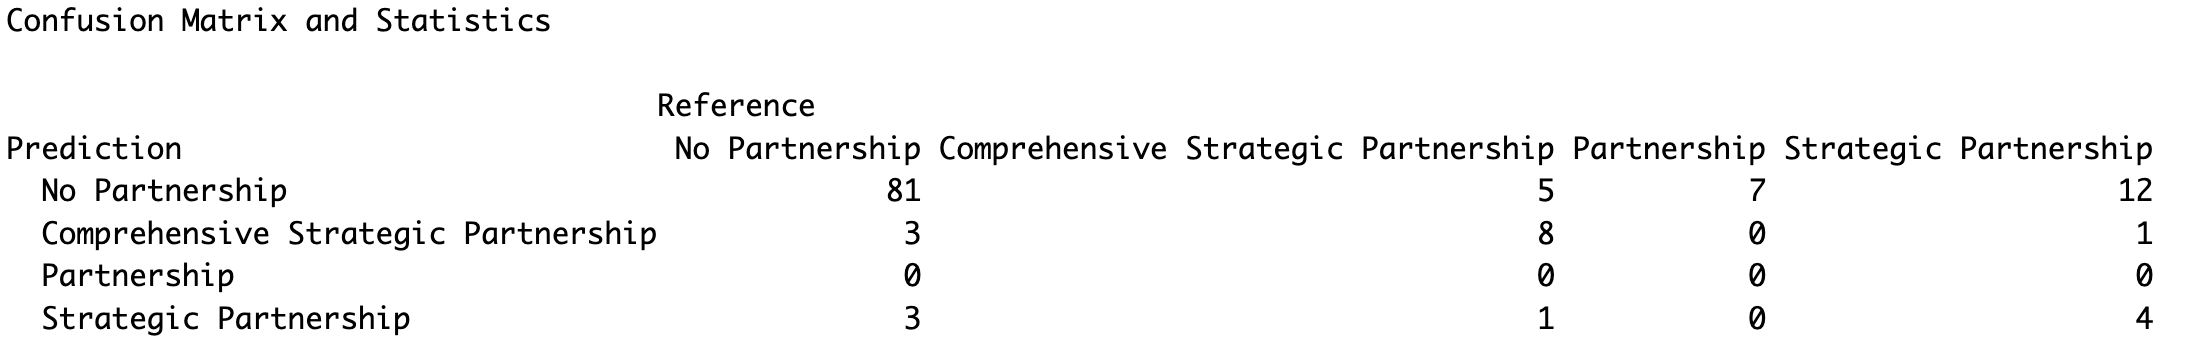
\includegraphics[width=1\linewidth]{cm_unordmodel1.png}
\end{figure}

\begin{figure}[H]
    \centering
    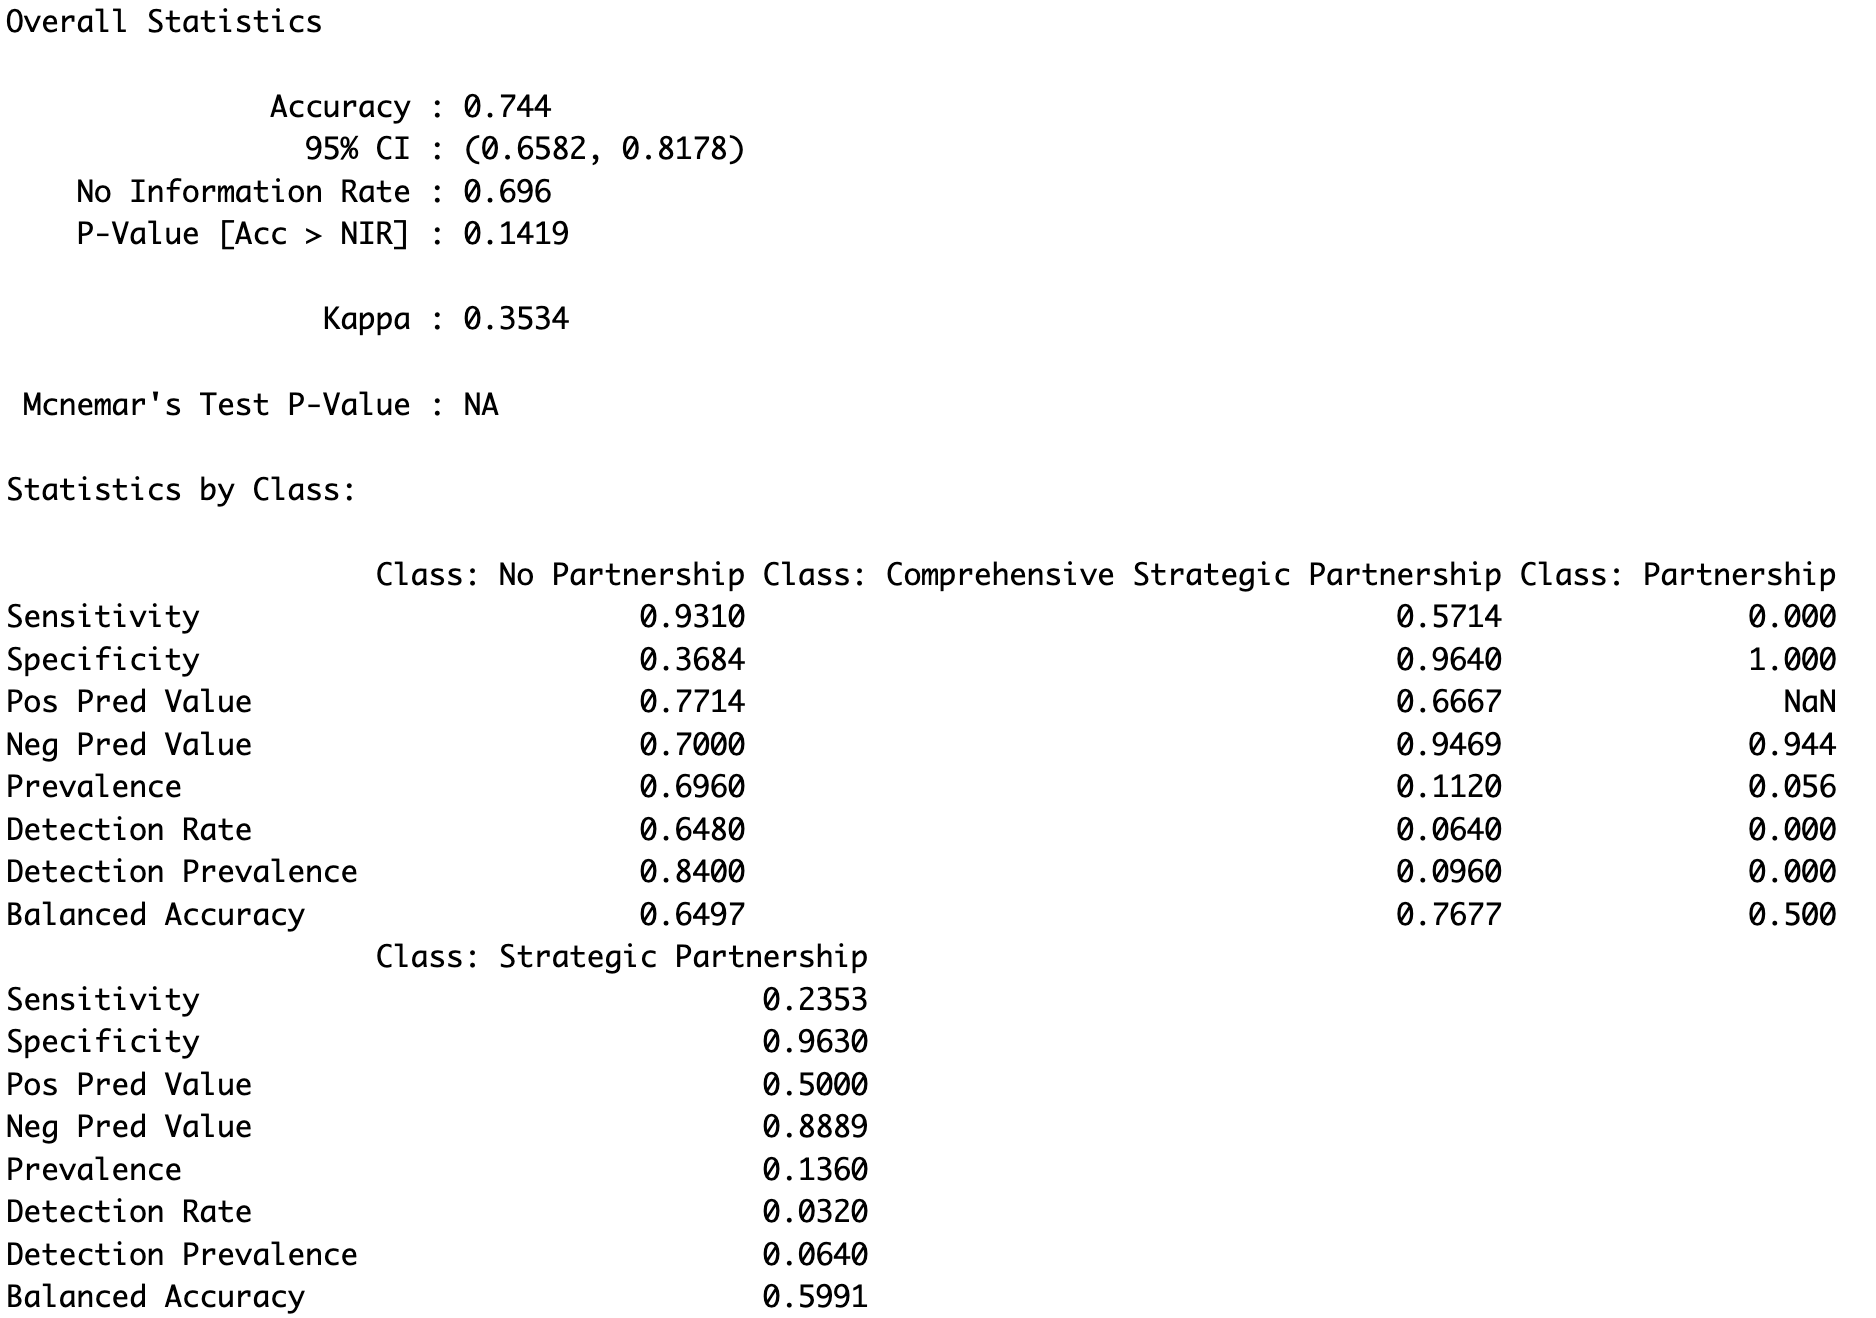
\includegraphics[width=1\linewidth]{cm_unordmodel2.png}
\end{figure}

\lstinputlisting[language=R, firstline=183, lastline=201]{Twist_Lee_MS.R} 

\begin{figure}[H]
    \centering
    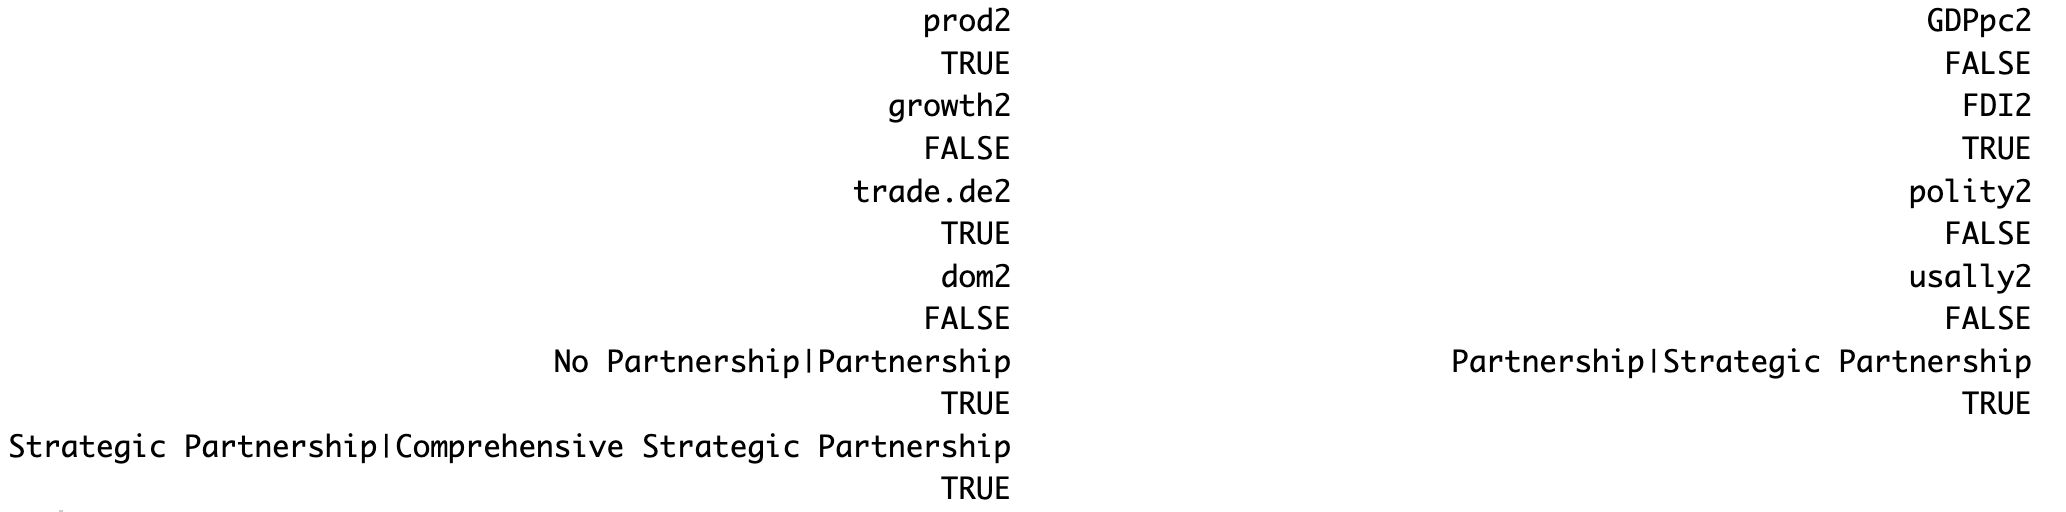
\includegraphics[width=1\linewidth]{pvalues_ord.png}
\end{figure}

\lstinputlisting[language=R, firstline=203, lastline=208]{Twist_Lee_MS.R} 

\begin{table}[H]
\centering 
\caption{Ordered Model (exponentiated)} 
\label{} 
\begin{tabular}{@{\extracolsep{5pt}}lc} 
\\[-1.8ex]\hline 
\hline \\[-1.8ex] 
 & \multicolumn{1}{c}{\textit{Dependent variable:}} \\ 
\cline{2-2} 
\\[-1.8ex] & Partnership Level \\ 
\hline \\[-1.8ex] 
 Oil production & 1.124$^{**}$ \\ 
  & (0.057) \\ 
  & \\ 
 GDP per capita & 0.694 \\ 
  & (0.256) \\ 
  & \\ 
 GDP growth & 0.958 \\ 
  & (0.086) \\ 
  & \\ 
 FDI inflows & 1.324$^{***}$ \\ 
  & (0.078) \\ 
  & \\ 
 Trade importance & 6.095$^{**}$ \\ 
  & (0.745) \\ 
  & \\ 
 Level of democracy & 0.953 \\ 
  & (0.050) \\ 
  & \\ 
 Domestic conflict & 1.155 \\ 
  & (0.131) \\ 
  & \\ 
 US ally & 0.841 \\ 
  & (0.678) \\ 
  & \\ 
\hline \\[-1.8ex] 
\textit{Intercepts} \\
\hline
\hline
No Partnership|Partnership & 77.138**  \\
Partnership|Strategic Partnership & 118.238**  \\
Strategic Partnership|Comprehensive Strategic Partnership & 513.783** \\
\hline
Observations & 125 \\ 
Log Likelihood & $-$90.19376 \\ 
Residual Deviance & 180.3875 \\
AIC & 202.3875 \\ 
BIC & 233.499 \\ 
\hline 
\hline \\[-1.8ex] 
\textit{Note:}  & \multicolumn{1}{r}{$^{*}$p$<$0.1; $^{**}$p$<$0.05; $^{***}$p$<$0.01} \\ 
\end{tabular}
\end{table}

\newpage
\lstinputlisting[language=R, firstline=210, lastline=215]{Twist_Lee_MS.R} 

\begin{figure}[H]
    \centering
    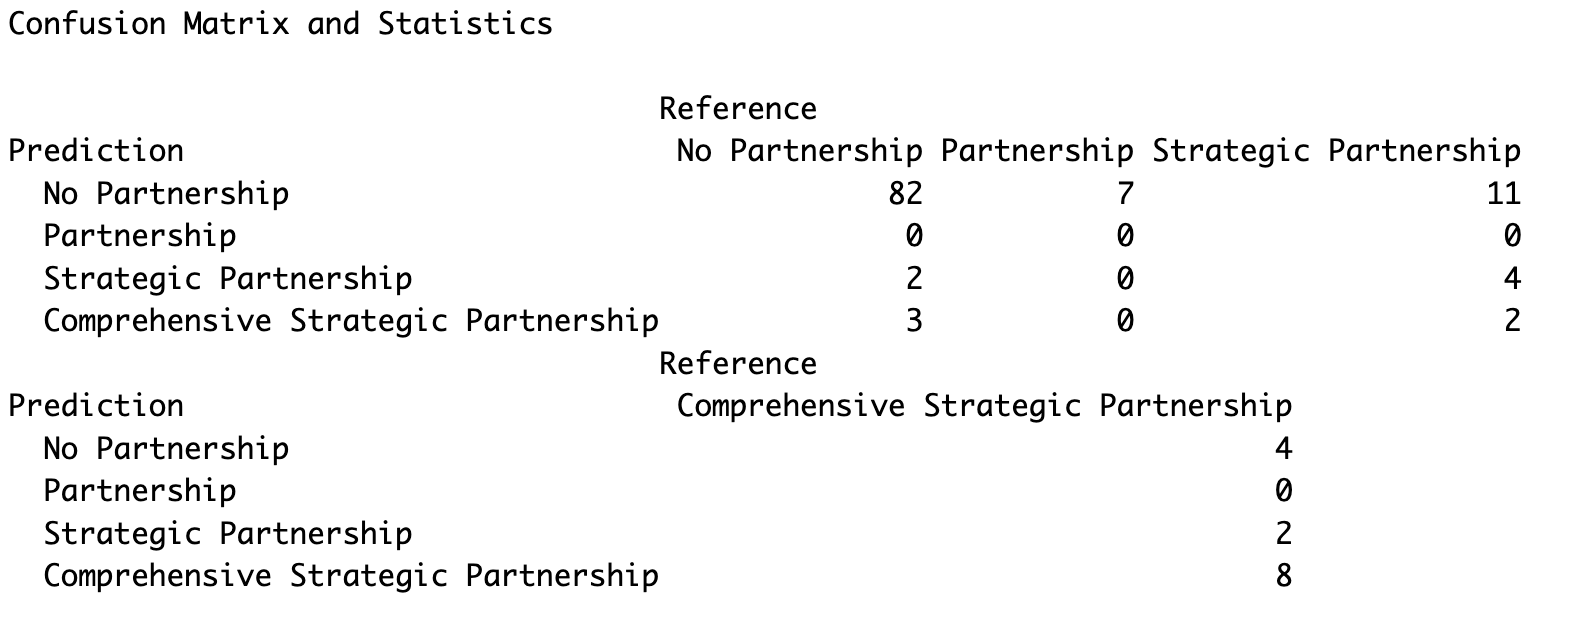
\includegraphics[width=1\linewidth]{cm_ordmodel1.png}
\end{figure}

\begin{figure}[H]
    \centering
    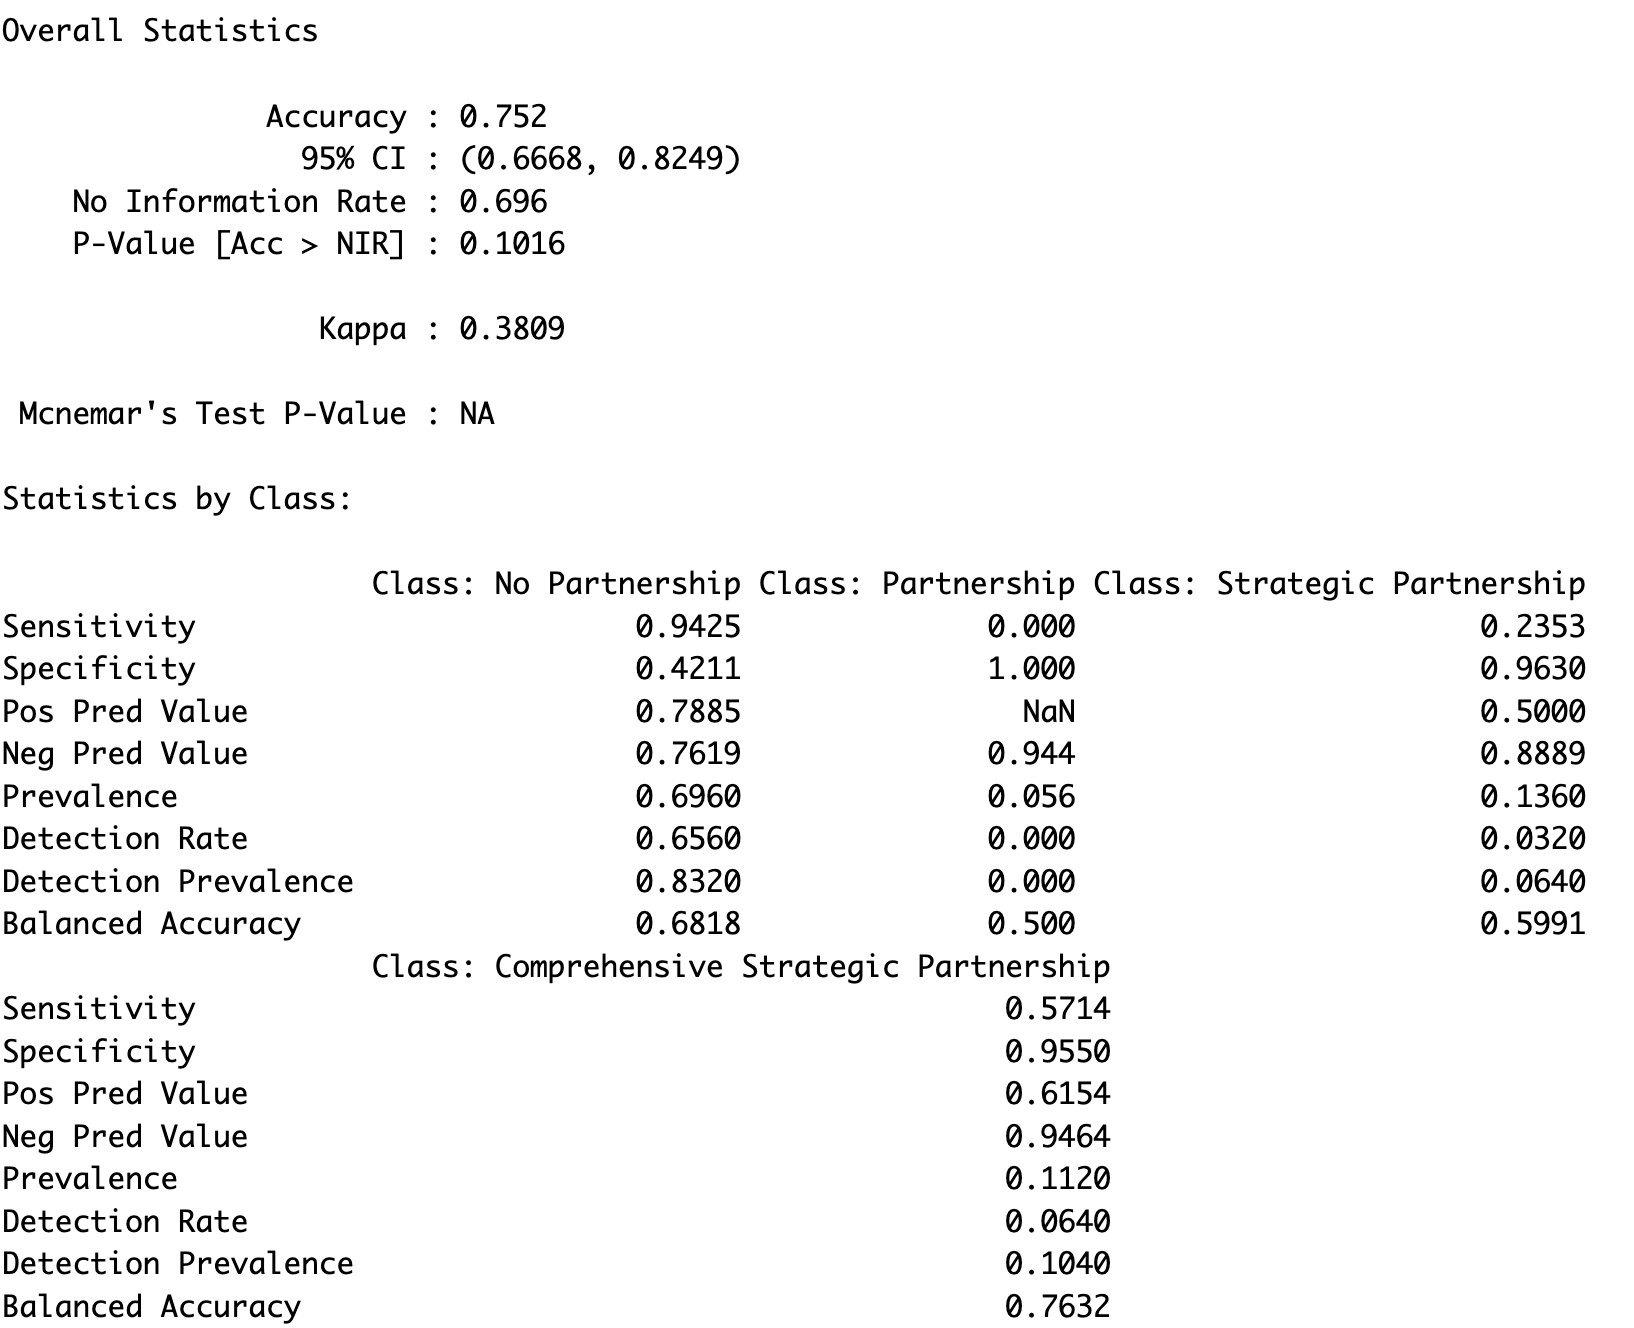
\includegraphics[width=1\linewidth]{cm_ordmodel2.png}
\end{figure}

\lstinputlisting[language=R, firstline=217, lastline=221]{Twist_Lee_MS.R} 
\begin{verbatim}
[1] 166.5255
[1] 180.3875
[1] 111.0911
\end{verbatim}

\lstinputlisting[language=R, firstline=223, lastline=226]{Twist_Lee_MS.R} 
\begin{verbatim}
[1] 129.0911
[1] 220.5255
[1] 202.3875
\end{verbatim}

\lstinputlisting[language=R, firstline=228, lastline=231]{Twist_Lee_MS.R} 
\begin{verbatim}
[1] 154.5459
[1] 296.89
[1] 233.499
\end{verbatim}

\lstinputlisting[language=R, firstline=233, lastline=234]{Twist_Lee_MS.R} 

\begin{figure}[H]
    \centering
    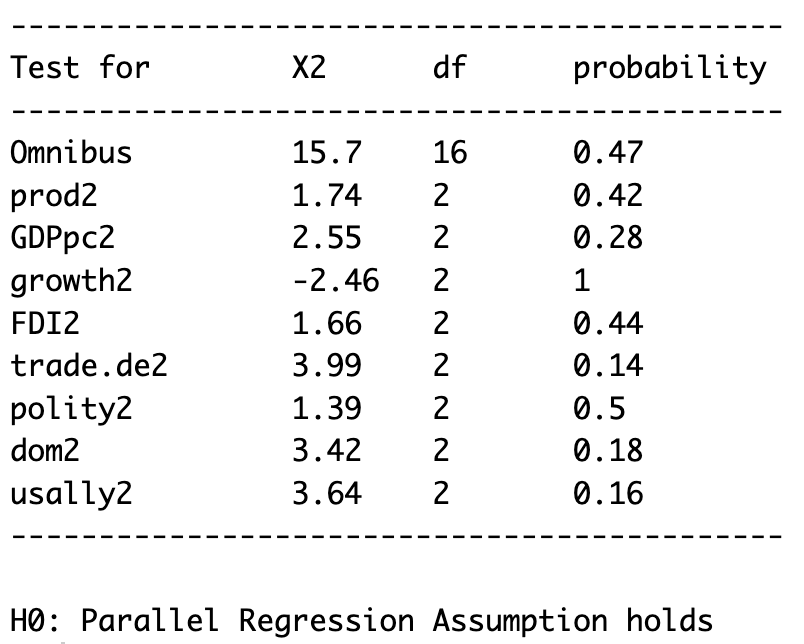
\includegraphics[width=0.5\linewidth]{brant.png}
\end{figure}

\newpage
\section{References}

\noindent Lee, C. (2019). China’s Energy Diplomacy: Does Chinese Foreign Policy Favor Oil-Producing Countries? \textit{Foreign Policy Analysis}, \textbf{15}(4), 570–588. \url{https://doi.org/10.1093/fpa/orz011} \\

\vspace{0.25cm}

\noindent Lee, C. (2023). "Replication data for 'China's Energy Diplomacy: Does Chinese Foreign Policy Favor Oil Producing Countries?'" [Data set]. Harvard Dataverse. \url{https://doi.org/10.7910/DVN/7E3O5P}, V1, UNF:6:x+exuF4WVfknqWQhUWz4MQ== [fileUNF].

\end{document}
